\documentclass[onecolumn,10pt]{IEEEtran}

\usepackage{graphicx}
\usepackage{siunitx}
\newcommand{\myroot}{../}
\newcommand{\Later}{\textbf{Later.}}

\title{Autonomous Drone Racing}
\author{A.~Credle and D.~Evangelista\thanks{Authors are with the United States Naval Academy, Department of Weapons, Robotics, and Control Engineering}}
\date{today}

\begin{document}
\maketitle

\begin{abstract}
Autonomous racing drones are not only beneficial to the drone racing sport, but also in autonomous vehicles and in military drones flying through windows, chimneys, etc. Research in this field is often based around either race gate recognition or flight controls, but this project will incorporate both. We will create a process for a drone to modify its given flight path based on the visual recognition of the gate in order to fly through the gate. The processor will identify the gate, locate it in relation to the drone’s current path, and modify the path to fly through the gate. This project will demonstrate this process by using simulations and physical experiments. Simulations will consist of individual tests of recognition, location, and path modification processes, and then tests for all three together. Physical experiments will test all three process together in a real environment. Success will be measured by the difference in distance between the path and the center of the gate, as well as the difference in trajectory at the same point. The total cost of the project is \$29,166- with \$1086 of that being new equipment. This project is scheduled to have the coding and simulation done within the first semester and physical experiments done by the end of the second. The biggest risk involved is with the drones crashing, so the physical experiments have more time than simulations to ensure safety. If successful, this will be the first step in creating an autonomous racing drone at USNA.
\end{abstract}

\section{Background and motivation}
The concept of drone racing is straightforward: a group of people fly unmanned aerial vehicles (UAV) through gates, the first one to the finish line wins. The UAVs, or drones, come in a variety of sizes, ranging from an inch in diameter to over a foot, and are flown through communication with a remote controller. Races can take place in a variety of conditions including time of day and location. Gates can be configured in an unlimited number of patterns and often come in circular or rectangular form, though they are not limited to these shapes. Limitations are often placed on the power and size of drones that are raced, as owners are often expected to bring their own equipment. While the concept of racing is not new, drone racing is one of the fastest growing sports in the world (CITE). There are no limitations on age, gender, ethnicity, or physical prowess, making drone racing available to everyone.
\begin{figure}
\caption{Two drones racing}
\label{fig1}
\end{figure}

The concept of autonomous drone racing is even newer, though its potential goes beyond that of its sport. In concept, a human drone racer goes through a series of ques and maneuvers to race the drone. If these ques and maneuvers are broken down into systematic steps, it is possible to automate the process and have the drone fly itself through the course. In modern autonomous vehicles, the specific location of the vehicle is often known, through GPS, a tracking system, etc. While this method of localization works for vehicles with static environments, it does not take into account the location of its surrounds, or the vehicles location in relation to specific objects. 

By mixing both an assumed path and gates for the drone to fly through, the exact location of the drone is not required; its relative location to the gates is all that is needed to fly a successful race. This concept will be critical for future autonomous systems, such as self-driving cars, that are required to navigate based on an assumed path mixed with the vehicles relative to the environmental objects or barriers (Fig. 1). For cars, the environmental objects would include lane lines, other vehicles, curbs, objects in the road, etc. By integrating objects of the environment into the core of the navigation process, autonomous vehicles will be able to keep both passengers, pedestrians, and wildlife safe. Autonomous vehicles of the future must be able to navigate based on both an assumed path and a relative location in order to efficiently and safely navigate dynamic environments.  
\begin{figure}
\caption{An autonomous car sensing its environment}
\label{fig2}
\end{figure}

As the first autonomous drone-racing project at USNA, this will open the door to future drone research for midshipmen. EW281 and EW282 provide opportunities for midshipmen to experiment with drones on a hardware and flight-testing level, but this project will allow for future drone development on the software and autonomy level. Additionally, this research is only the first step in creating a fully autonomous racing drone that rivals a human’s performance. Future steps include path optimization, recognition with visual uncertainties, racer collision avoidance, etc. This research will be one small step in the larger picture of fully autonomous drone racing.




\section{Problem statement}
Given a three-dimensional flight path, drone accelerometer readings, and the image of a drone-racing gate in a three dimensional environment, this research intends to begin the process of developing autonomous drone flight through a drone-racing course. Given a three-dimensional path that does not fly through the gate, we will find and test the feasibility of a guidance system that creates a similar path that does. This system will be tested by placing a small quadrotor in multiple scenarios in relation to a race gate(s), with varying pre-determined paths, and directing the guidance system to fly the drone through the race gate(s). Success of this system is based on the ability to autonomously correct the path and fly the drone through the center of the gate without contact. This will be measured by the difference in distance between the path at its intersection with the gate, and the center of the gate. The competing objective will be to maintain the same trajectory at the intersection with the gate as if the path had not been modified. The final output of this project will a guidance system that could be implemented on any racing drone with a camera and IMU and fly through race gates autonomously.

\begin{figure}
\caption{Depiction of flight path correction (original path in green, new path in blue, trajectory at gate intersection as red arrow, gate intersection point as red dot)}
\label{fig-problem-statement}
\end{figure}

% OLD REMOVED BY AC 3 MAY 2019
%\begin{figure}[h]
%\begin{center}
%\includegraphics[width=4in]{\myroot/figures/racegate-intro.png}
%\end{center}
%\caption{A quadcopter drone flying through a racing gate.}
%\label{fig-problem-statement-1}
%\end{figure}
%




\section{Literature review}
This paper is the one of the first developments of a drone autonomous flight program at USNA, so the background research encompasses papers that focus on multiple aspects of autonomous flight. The main categories that these papers fall into include navigation, flight controls, and visual recognition. This research focuses on the visual recognition of the gate, but these other two categories are necessary for the background research because they affect the performance of visual recognition and are necessary for basic demonstration. 

In order to understand the movement patterns of the drone, \cite{svacha2017improving} provides a set of equations that could be used to accurately model the induced drag and thrust forces. These equations were derived from proofs using properties of physics, and then the coefficients were identified through flight experimentation. This allows provides suitable estimations for the forces acting on the drone, which allows for control of the drone through the gate. This is connected to \cite{loianno2017estimation}, which created a state equation set that could accurately model the movement of a small drone with aggressive flight. By determining these equations through modeling and live testing, these state equations can be coupled with the flight force equations from \cite{svacha2017improving} to form an accurate estimate of the drones location. Coupling these with a flight controller will allow the drone to have a basic understanding of its location as compared to the general space. This research is centered around coupling visual servoing and preprogrammed flight paths, and in order to understand the drones relation to the preprogrammed flight path, \cite{svacha2017improving} and \cite{loianno2017estimation} provide an accurate location. 

While \cite{svacha2017improving} and \cite{loianno2017estimation} provide what is believed to be an accurate location of the drone in-flight, it’s location in relation to the preprogrammed flight path isnt always certain. \cite{florence2018nanomap} provides the groundwork for a concept known as ``nano mapping'', which refers to modeling a 3D data structure depicting obstacles around the drone. This technique is different from a traditional mapping approach because tradtional mapping is based of a common world frame. \cite{florence2018nanomap} is based solely on the frame of the drone, allowing for a calculatable uncertainty to enter trajectory planning. This concept is also crucial to the development of this research because the coupled flight path planning approach requires both the common world frame and the drone world frame.

Different methods for seeing the world around the drone exist, including range finding technology (used for altitude measurements), single camera, and multi camera approaches. \cite{loianno2017estimation} is based on a single camera approach, while \cite{zhilenkov2018use} found that a three camera setup was optimal for uncertain terrains. \cite{zhilenkov2018use} is based on autonomous navigation of drones in a wooded area where the location of the trees is unknown before flight. The drone does not have a preprogramed path, but rather has a program to recognize key features along a route and to estimate the likelihood of needing to turn. While the racecourse for this research is assumed to be known, a single camera approach will be utilized for hardware simplicity; estimating the likelihood that the computer is seeing a gate, however, may be utilized in this research. If a neural network could be constructed to follow a path through a forest, a similar neural network could be formed to fly through an aerial path.

One of the main challenge that arises with flying through the gate is recognizing multiple gates. In small drone racing courses, it is likely that the drone will be able to see multiple gates within its field of view. \cite{jung2018perception} worked through this problem and found resonable neural network perameters to mitigate this issue. By assuming the next gate in the racecourse would be the largest gate in the drone camera view (using a single camera approach), \cite{jung2018perception} removed the nueral network layer of all image analysis and left only the recognition of the largest circle gate. By removing this process in the image analysis, \cite{jung2018perception} found a significant increase in processing power while only reducting the accuracy of gate recognition by less than \SI{10}{\percent} (\SIrange{464}{34}{\milli\second} reaction time, \SIrange{82.4}{75.5}{\percent}).

The other main challenge that arises after recognizing the proper gate to fly through is implementing a visual servoing program to direct the drone through the gate. \cite{jung2018direct} created a process of gate recognition that located the center of the gate in relation to the location of the center of the cameras view and redirecting the drone towards the center of the gate. This background research is the closest process to the research in this paper, as it specifies a visual recognition process that is simplified into the computational level of an inflight processor.

While many of these papers are useful in the development of an autonimous drone, it should be noted that there lacks a consistancy among drone researchers in the underlying assumptions. As described earlier, some researchers utilize a single camera operating system, while others use multi-camera systems, and even some include range finding technology. Many of the subjects of these papers devled into different subsections of drone autonomy, so it is reasonable that their methods varied. For research such as \cite{svacha2017improving}, \cite{loianno2017estimation}, and \cite{florence2018nanomap}, their research was more for drone flight in general, so this critique doesn’t apply as much as it does for projects such as \cite{zhilenkov2018use}, \cite{jung2018perception}, and \cite{jung2018direct}, which had varying sensor and visual capabilities. As the latter three projects had more to do with direct visual recognition, it would have been more advantageous for the autonimous drone community had the projects been embarked on in a similar manner.

These projects center around the research in this proposal in two ways: by giving basic flight control and navigational equations to use in baseline location estimations and flight controllers, and by providing simplistic approaches to visual recognition to model my approach. While my approach uses both a whole world frame and a drone view frame to form a novel approach to gate recognition, many of the approaches depicted in \cite{zhilenkov2018use}, \cite{jung2018perception}, and \cite{jung2018direct} can be used to model a realistic approach to melding the two frames. This project will take these simplistic approaches and form a simple and novel approach to visual gate recognition.








\section{Demonstration plan}
%IV. DEMONSTRATION PLAN
%Simulation- isolate and test each part, bring together for experiment
%In this project, it is important to ensure that factors not related to gate recognition and visual servoing do not hamper the performance of the drone. This research intents to recognize, locate, and fly through a drone-racing gate, so all other aspects of drone flight will be controlled. Initial testing will be conducted in drone flight simulators to allow for repeatability and a constant testing environment. This will ensure that gate recognition and visual servoing processes can be refined and optimized before moving to actual flight-testing.
%In order to demonstrate the effectiveness of the recognition and flight-path correction processes, a mix of simulations and experiments will required. First, simulations will be run to test each of the “recognize, locate, and correct path” process. Secondly, a simulated course will be run in order to demonstrate ideal drone capabilities with mixed gate recognition and path correction programming.
%Last, a physical experiment with a small, single camera quadcopter with an internal IMU will with a variety of racecourse configurations to ensure its practicality with real world environmental factors. Experimentation will occur indoors so that these factors will be minimal and repeatable. 

\Later\ In this project, it is important to ensure that factors not related to gate recognition do not hamper the performance of the drone. With small quadcopters performing advanced maneuvering, it can be difficult to predict and measure its exact movements, which could negatively affect this projects ability to test gate recognition capabilities. While not optimal for a project focused on practicality, initial testing will be conducted in drone flight simulators. This will ensure that gate recognition processes can be focused on before moving to actual flight-testing.

In order to demonstrate the effectiveness of the gate recognition process, a mix of simulations and experiments will required. First, simulations will be run to give the AI enough examples to test its understanding of what a gate looks like, so the same simulation can be used to show the AIs theoretical accuracy. Secondly, a simulated course will be run in order to demonstrate ideal drone capabilities with mixed flight and gate recognition programming. Last, a physical experiment with a small, single camera quadcopter with an internal IMU will be sent through a variety of racecourse configurations to ensure its practicality.

%\subsection{Mathematical analysis}

\subsection{Simulation or computational studies}
%    A. Simulation or computational studies
%WIP
%As stated previously, simulation will be relied on heavily before moving into experimental work. This is to ensure that any unknown external factors do not interfere with the “recognize, locate, and fly” process. This is critical because it allows for repeatable testing without varied results. Environmental factors are difficult to measure, so simulation testing allows for those factors to be controlled or removed entirely. In addition, testing in simulation will allow for quick specific adjustments. This allows for testing to be run at a faster rate than a physical test.
%Simulation testing for the first two sections of the demonstration is necessary because of its control, replicability, and generality. In the drone flight simulators, a myriad of flight controls can be controlled with the click of a button. Every movement of the drone will be calculated and ideal. This is optimal for initial demonstrations for two reasons. First, it allows for exact movements, so the drones flight can be programmed simply. For example, if gates are introduced into the simulation directly in front of the drone, the simulation can be programmed to fly the drone straight through the gates without having to worry about altitude loss, wind factors, drag, etc. On a very basic level, the drone can be programmed to fly a perfectly straight line. While this is not realistic to real world environments, it is useful for initial gate recognition. Secondly, this test can be replicated thousands of times an hour. If thousands of test runs are collected, we can product an accuracy rating for the gate recognition processes, and failed test runs can be analyzed for process alterations.
%While recognizing a gate head on in a simulated environment may not be incredibly difficult, a new challenge will be added to test the recognition software. The bigger challenge is having the drone recognize gates from non-ideal angles. In cases where a drone approaches a gate at an increased angle, it is assumed that the recognition processes will struggle. Identifying a pure square is easy, however recognizing a small rectangle and accurately predicting an approach angle that allows the drone to fly through the gate without hitting either gate edge is more challenging. By running simulations where thousands of angles can be tested, this allows for a complete understanding of the image processing and visual servoing capabilities. This allows for complete control of the drones flight, and can be replicated thousands of times over. By creating a general understanding of the drones response to different situations, troubled situations can be mitigated and a more accurate physical experiment can be implemented.


As stated previously, simulation will be relied on heavily before moving into experimental work. This is to ensure that any unknown external factors do not interfere with the gate recognition process. This is critical because if there are adjustments required upon final testing, testing in simulation will allow for quick specific adjustments. In addition, this allows for testing to be run at a speed exponentially faster than a physical test.

Simulation testing for the first two sections of the demonstration is necessary because of its control, replicability, and generality. In the drone flight simulators, a myriad of flight controls can be controlled with the click of a button. Every movement of the drone will be calculated and ideal. This is optimal for initial demonstrations for two reasons. First, it allows for exact movements, so the drones flight can be programmed simply. For example, if gates are introduced into the simulation directly in front of the drone, the simulation can be programmed to fly the drone straight through the gates without having to worry about altitude loss, wind factors,drag, etc. On a very basic level, the drone can be programmed to fly a perfectly straight line. While this is not realistic to real world environments, it is useful for initial gate recognition. Secondly, this test can be replicated thousands of times an hour. If thousands of test runs are collected, we can product an accuracy rating for the gate recognition processes, and failed test runs can be analyzed for process alterations.

While recognizing a gate head on in a simulated environment may not be incredibly difficult, a new challenge will be added to test the recognition software. The bigger challenge is having the drone recognize gates from non-ideal angles. In cases where a drone approaches a gate at an increased angle, it is assumed that the recognition processes will struggle. Identifying a pure circle is easy, however recognizing a small ellipse and accurately predicting an approach angle that allows the drone to fly through the gate without hitting either gate edge is more challenging. By running simulations where thousands of angles can be tested, this allows for a complete understanding of the image processing capabilities. This, again, is not the most realistic test, but it allows for complete control of the drones flight, and can be replicated thousands of times over. By creating a general understanding of the drones response to different situations, troubled situations can be mitigated and a more accurate physical experiment can be implemented.

\subsection{Experimental work}
%    B. Experimental work
%WIP
%Crabbe ai, human testing
%The second phase of demonstration for this project includes proof-of-concept experiments of a drone flying through single and multi-gate racecourses. First, a single gate course will be created in order to test “locate, identify, and modify path” with real world factors. The drone will be set to take off from a flat surface, recognize a gate placed in front of it, modify its flight path to fly through the gate, and then land on a flat surface. The test will then be modified by moving the gate from directly in front of the drone to different locations so the drone can be shown recognizing and flying through different approach angles. Next, a multi-gate course will be created (2-5 gates) in which the drone will fly through the gates in sequential order. Sequential order is important as it shows the recognition programs capability of distinguishing which gate is closer, in turn recognizing the correct order of gates. While initial multi gate testing will be conducted with the gates in a straight line, the gates will eventually be configured in curved and staggered patters (see Fig. 1 and Fig. 2 below). These tests are the closes to drone racing that this project will go, as demonstrating multi-gate recognition is subsequent for basic drone racing. In the future, this project could be utilized for a high speed-racing drone, which would need better flight recognition capabilities (seeing gates at long distances or flying towards gates outside of the cameras line of sight), but for this project, simple gate testing will be sufficient.

The second phase of demonstration for this project includes proof-of-concept experiments of a drone flying through single and multi-gate racecourses. First, a single gate course will be created in order to test basic gate recognition processes alongside flight controllers. The drone will be set to take off from a flat surface, recognize a gate placed in front of it, fly through the gate, and then land on a flat surface. The test will then be modified by moving the gate from directly in front of the drone to different locations so the drone can be shown recognizing and flying through different approach angles. Next, a multi gate course will be created (2--5 gates) in which the drone will fly through the gates in sequential order. Sequential order is important as it shows the recognition programs capability of distinguishing which gate is closer, in turn recognizing the correct order of gates. While initial multi gate testing will be conducted with the gates in a straight line, the gates will eventually be configured in curved and staggered patters (see Figures~\ref{fig-gate-style-1} and \ref{fig-gate-style-2} below). These tests are the closes to drone racing that this project will go, as demonstrating multi-gate recognition is subsequent for basic drone racing. In the future, this project could be utilized for a high speed-racing drone, which would need better flight recognition capabilities (seeing gates at long distances or flying towards gates outside of the cameras line of sight), but for this project, simple gate testing will be sufficient.
\begin{figure}
\caption{Depiction of multi-gate racecourse style 1}
\label{fig-gate-style-1}
\end{figure}

\begin{figure}
\caption{Depiction of multi-gate racecourse style 2}
\label{fig-gate-style-2}
\end{figure}

For the physical experiments, standard drone racing specifications will be maintained. Lockheed Martin currently has a drone racing competition, known as the AlphaPilot Challenge, which requires specific drone specifications (power supplies, drone size, motor power, etc.). As these specifications are published, they will be maintainedwithin this project, and it is assumed that these specifications will meet the requirements for powering, computing, and sensing within this project.

\subsection{Property measurement}
%C. Property Measurement
%The primary measurement for the simulation and experimental testing will be the deviation from the modified path and the target point in the plane of the gate. This will be measured using data collected from the simulation software and from the Optitrack system during the experimental testing. The competing measurement will be the difference in the trajectories between the original path and the modified path at the gate intercept points. This measurement will be a three-dimensional vector, so each individual vector part will be compared.  
%As this is only the first step in creating a fully autonomous racing drone, this project’s objective is not to produce a full speed autonomous racing drone. Previous research in the gate recognition field showed that at full speed (5 m/s), correct gate recognition with multiple gates in the field of view had a 75%-85% success rate. This project will be flying the drone at a much slower speed (.5 m/s), and initial experimentation will use a lit gate in a dark room. This is to ensure gate recognition is not hampered by the environment so that it can be assumed the gate will be recognized. With this assumption, gate recognition will not be measured as it has been with previous research. Further measurements can be done with future capstone groups testing this process at higher speeds. 

As this is the first phase within the many steps required for functional autonomous drone racing, it is assumed that the results from this project will be close to the results of current research. As seen in \cite{jung2018perception}, the accuracy of AI integrated gate recognition using large off-board computers was found to be between \SIrange{75}{85}{\percent} gate recognition accuracy. This data was taken at full flight speeds (\SIrange{4}{5}{\meter\per\second}), while this project is not focused on speed, so it is assumed we will have similar accuracies. In order to compare our results to those of other researchers in the gate recognition field, a gate recognition accuracy measurement is necessary. This is comprised of the number of gate correctly recognized in the proper order divided by the number of gates the drone is presented.

\subsection{Technical risks and mitigation}
%D. Technical risks and mitigation
%The main technical risk involved with this research is processing speed. In the event that the gate recognition and path modification processing is too complex and lags, the drone will not be able to complete its course. In order to mitigate this risk, the approach to building the program will be to build from simplicity, rather that simplifying something complex. This will allow for the simplest and fastest processing, mitigating the risk of lag.
%Due to the innate troubles with high-speed drone flight, there is always the risk of crashing a drone. In our experiments, we plan to minimize this risk by keeping speeds significantly lower than racing speed (.5 m/s vs 5 m/s). In addition, drone flight will be at low altitudes, so in the event a hard shutoff is required, the drone will only fall a foot onto a carpeted floor. This should allow for a safety shutoff without damaging the drone. 
%The only other issue that may arise is low battery life, which will be mitigated by purchasing multiple drones and batteries, as accounted for in the budget section.
%

Due to the innate troubles with high-speed drone flight, there is always the risk of crashing a drone. In our experiments, we plan to minimize this risk by keeping speeds significantly lower than racing speed (\SIrange{0.5}{5}{\meter\per\second}). In addition, there is a collection of drones from past swarm projects available, so excess batteries and drones are available in the event that batteries die or drones crash and break. While there may be technical issues with building drones specific to the AlphaPilot Challenge, the instructions provided with the drone building class at USNA are easily accessible, so issues with drone building and drone flight should be minimal. The only other issue that may arise is low battery life, which will be mitigated by the batteries available at USNA, or will be budgeted for (this will be known by the budget section due date).

%\subsection{Time risks and mitigation}
%F. Time risks and mitigation
%	The timeline for this project can be found in encl. 1. The main portions of the projects include relearning python, writing code, integrating inputs, simulation testing, single gate experimental testing, and multiple gate experimental testing. The biggest time risk is in the coding and input integration. While not ideal, experimentation and simulation can be done simultaneously; however, both require working code. If the control algorithm takes longer to create than planned, it would push back simulations and experimentation. This is mitigated by allow more than ample time to run physical experiments, so if both simulation and experimental testing are pushed back, experimental testing can take a time hit without suffering.
%


%\subsection{Justification of high risk activities}
%G. Justification of special high risk activities
%This research will be conducted using Python, as it allows for high level control of the gate recognition and path correction processes. While learning a language is risky, it is advantageous for this project because most other drone flight projects on the yard utilize Python, so cross-referencing will be much easier if I use the same language. It can also be assumed that Python is likely the best language to use for this type of project since other projects are using it as well. In addition, I have completed SY202, the introductory course for Cyber majors at USNA. This course taught the basics of the Python language, so I feel confident in my python coding abilities, and will likely only need a refresher in the language. The first 3 weeks of the timeline have been dedicated to refreshing on python, which should be sufficient to complete this project.

%\subsection{Budget}
%H. Budget
%In order to conduct the physical experiment demonstrations, a set of drones and race-gates are necessary. The drone required a single camera, an IMU, and a flight controller. The DJI Tello drone was selected as it has all of the required parts and is easily programmable. The DJI Tello is already being used on the Yard for Capstone projects, so there are readily available resources to help in the event that the drone breaks or malfunctions. In addition, the Vortex 180 drone was selected because it is a standard sized racing drone and it fits all of the requirements for this research. This drone will allow the research to get as close to true drone racing conditions as possible. Finally, the TBS gates were selected as they are sized for indoor drone racing and come with programmable lights. The lights allow for easy gate recognition during the first stages of experimental work as the lights in the testing room can be turned off and the gate lights turned on. This removed the background environment from the drone’s field of view, making gate recognition easier. The total labor, overhead, and material costs can be seen in Table 1, and the breakdown of the out of pocket costs for materials can be seen in Table 2.
%
%Table 1: Labor, overhead, and materials costs
%
%
%Table 2: Out of pocket costs
%
%
%

%\begin{table}[hb]
%\caption{Budget}
%\label{table-budget}
%\end{table}

\section{Conclusion}
In conclusion, this research will create a process for a drone to modify its flight path based on the visual recognition of racing gates. This is the first steps in the process to create a fully autonomous racing drone. Future steps will include path optimization and processing optimization. The process for this research will identify the gate, locate it in relations to the drone, and modify the flight path to fly through the gate. The processor will have a visual feed, the three dimensional acceleration data of the drone’s flight, and the pre-determined three-dimensional path. The process will output a new three-dimensional path for the drone to follow in order to fly through the gate. This project will demonstrate this process by using the Liftoff Flight Simulator and physical experiments to refine and optimize the program and measure results. Success will be measured by the accuracy of the new three-dimensional path as it passes through the gate. Accuracy is based on the difference in distance of the path and the center of the gate. The biggest risk involved with this research is damaging the drones during the experimental demonstrations, but this risk will be mitigated by extensive use of the simulator first. 

\section*{Acknowledgements}
\addcontentsline{toc}{section}{Acknowledgements}
We thank Prof Esposito, MIDN 2/C Ethan Marcello, and the EW502 class for helpful comments which were incorporated into this proposal.

\bibliographystyle{IEEEtran}
\bibliography{IEEEabrv,\myroot/references/credle}
%REFERENCES
%[1] J. Svacha, M. Kartik and V. Kumar, "Improving Quadrotor Trajectory Tracking by Compensating for Aerodynamic Effects," in International Conference on Unmanned Aircraft Systems (ICUAS), Miami, FL, USA, 2017.
%[2] G. Loianno, C. Brunner, G. McGrath and V. Kumar "Estimation, Control, and Planning for Aggressive Flight With a Small Quadrotor With a Single Camera and IMU," IEEE Robotics and Automation Letters, vol. 2, no. 2, pp. 404-411, 2017.
%[3] P. R. Florence, J. Carter, J. Ware and R. Tedrake, "NanoMap: Fast, Uncertainty-Aware Proximity Queries with Lazy Search over Local 3D Data," in CSAIL, Massachusetts Institute of Technology, Cambridge, MA, USA, 2018.
%[4] A. A. Zhilenkov and I. R. Epifantsev, "The Use of Convolution Artificial Neural Networks for Drones Autonomous Trajectory Planning," Faculty of Control Systems and Robotics, Department of Control Systems and Informatics, ITMO University, Saint Petersburg, Russia, 2018.
%[5] S. Jung, S. Hwang, H. Shin and D. H. Shim, "Perception, Guidance, and Navigation for Indoor Autonomous Drone Racing Using Deep Learning," IEEE Robotics and Automation Letters, vol. 3, no. 3, pp. 2539-2544, 2018.
%[6] S. Jung, S. Cho, D. Lee, H. Lee and D. H. Shim, "A Direct Visual Servoing-based Framework for the 2016 IROS Autonomous Drone Racing Challenge," Unmanned Systems Research Group, Department of Aerospace Engineering, Korea Advanced Institute of Science and Technology, Daejeon, Republic of Korea, 2017.
%





%
%\appendix
%\section{Gantt Chart}
%\Later\ Insert the Gantt chart here. Be sure the font is legible. Crop it tight, use landscape orientation and make it as large as possible.
%

%\begin{IEEEbiography}[{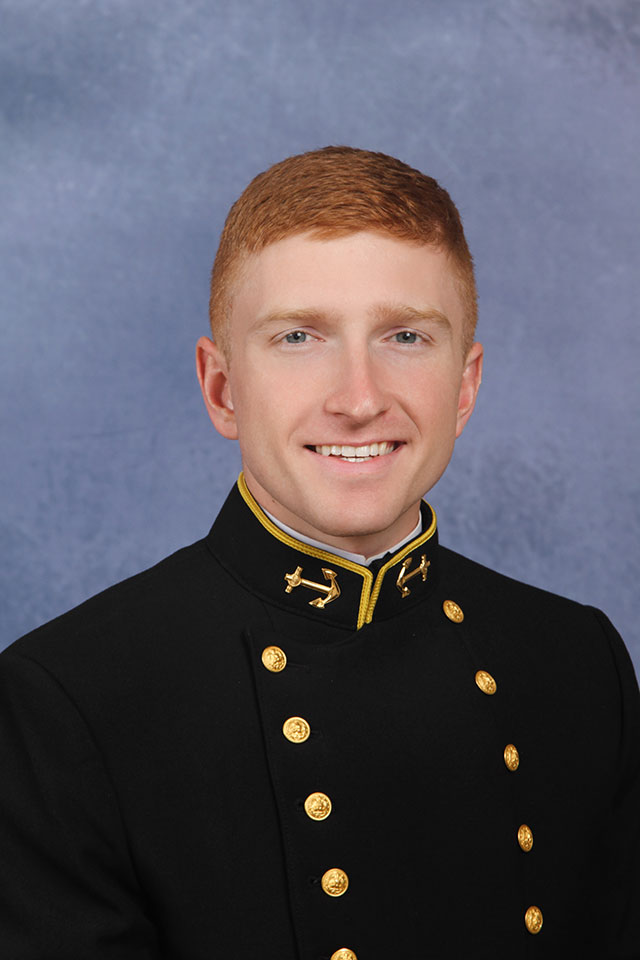
\includegraphics[width=1in,height=1.25in,clip,keepaspectratio]{\myroot/figures/M201260.jpg}}]{Austin Credle} is a midshipman at the United States Naval Academy majoring in Robotics and Control Engineering. Upon graduation, he hopes to service select as into either the pirate/privateer or blimp communities. 
%\end{IEEEbiography}
%
%\begin{IEEEbiography}[{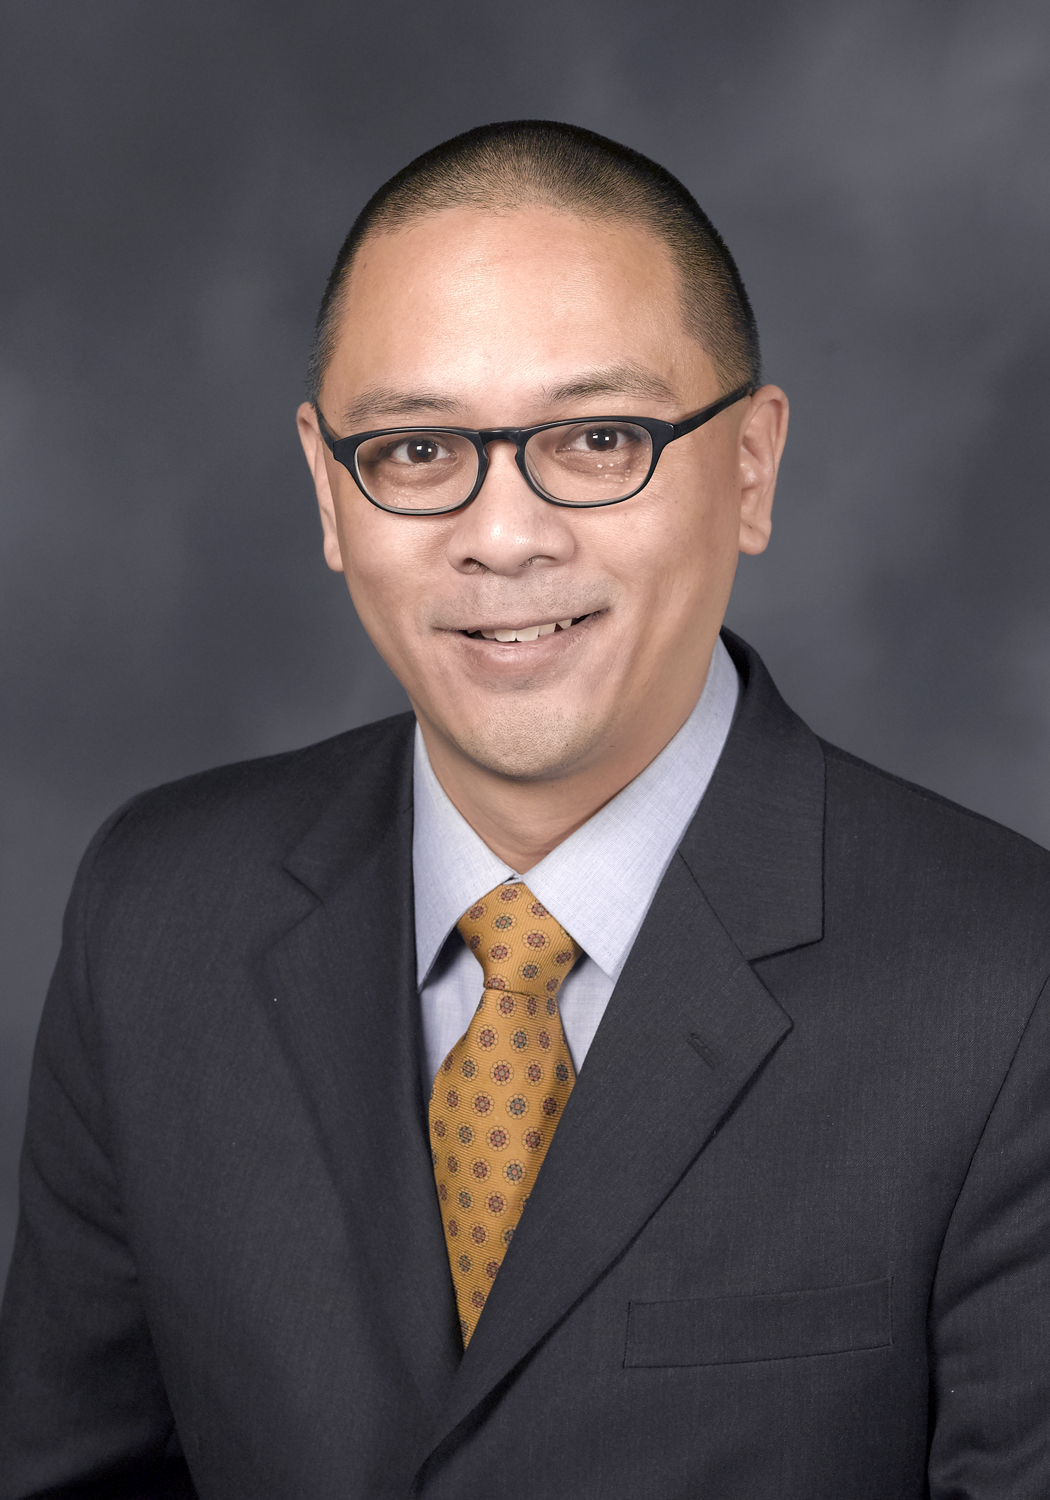
\includegraphics[width=1in,height=1.25in,clip,keepaspectratio]{\myroot/figures/evangelista_d_prof.jpg}}]{Dennis Evangelista} raises guide dog puppies. 
%\end{IEEEbiography}
%
\end{document}



%
%Left to do:
%Get research from wenberg, add to related works
%Budget- add cushion, conference, stretch goals
%Rework simulation and experimental demonstration
%Add citations to background research
%
%
%
%



